% !TEX root = SystemTemplate.tex

\chapter{Overview and concept of operations}

This system is for professors to test their students’ programs against test data contained in text files. The results of these tests will then be written to a text file for th user to evaluate the tested programs performance.

Title: Dr. Logar’s User Story As a professor I want to have a program compile, run, test, and evaluate the tests run on a program submitted to me by my students so that I no longer have to run each test case individually and evaluate them by hand.
The progam should compile and run a program against all test cases contained in files ending in ”.tst” within the current directory or within a subdirectory. In addition, it will evaluate the passes and fails of the program and log this in a text document for user review.
Titile: Revisions to make life  easier. It is also desired that this test suite runs all test files contained in a test directory against each program submitted by a student. Each student will have their own directory where the result file should be stored. 
Title: Automatic tests. As I am quite I would like to have the test suite generate its own tests so that I don't have to. It will store these tests in the tests subdirectory and generate the answer file for each test. 





\section{Scope}
The purpose of this project is to create a program that will run another program against test documents and output the 
results into another file forthe user. The program is specifically geared toward computer science professors for their use in 
grading student programs. This program will compile and run the submitted program imputting the test data. The results, which are saved to a text document, are evaluated and and percentage of pass/fail is also computed and saved in the
document.


\section{Purpose}
This system is designed in order to make it easier for professors to grade their students programs. The test files need only be 
in the same directory (or within a subdirectory) as the program to be compiled and run. Also, the output is to be detailed 
enough so that the user knows exactly which test cases passed and which failed.


\subsection{Program Compiler}
Though rather simple to code this is a mojor component because it depends on which system the program is running as to
how the program is compiled. This program is made to run using the gcc command.

\subsection{Test File Location}
Also a simple but necessary component to our system. The program is going to run every file ending in ".tst" within the same
directory as the progam itself. Therefore, searching the current working directory as well as every subdirectory is very 
important to ensure every test case is run.

\subsection{Test Case Evaluation}
Here is the most critical part of the program. This is where the tests are read in by our program and the results evaluated. 
Once evaluated the results are stored in a text file for the user to review. We will test various different possbile directory orderings as well as the ability to run against varying types of test cases.

\section{Systems Goals}
The goals of our system is to successfully compile and run a program with the test files in the directory. Then to output the result of the tests in a text file. It is also our goal to generate our own test cases for the user and generate cooresponding answer files.

\section{System Overview and Diagram}
The system flow is pretty simple. The program will walk through directories searching for test cases to run student programs on. With this resent update we have a specific file directory we expect. This program will be placed in the root directory. In this root directory will be a subdirectory for each student as well as a tests subdirectory, which will naturally store the tests. There will also be a golden.cpp in the root directory. This program, if prompted, will generate test cases and store them in the tests subdirectory and will use the golden.cpp to generate anwer files which will be placed in the root directory. Afterwards, the program will walk through the students directories and run their program against all the tests and give them a grade. 

\begin{figure}[tbh]
\begin{center}
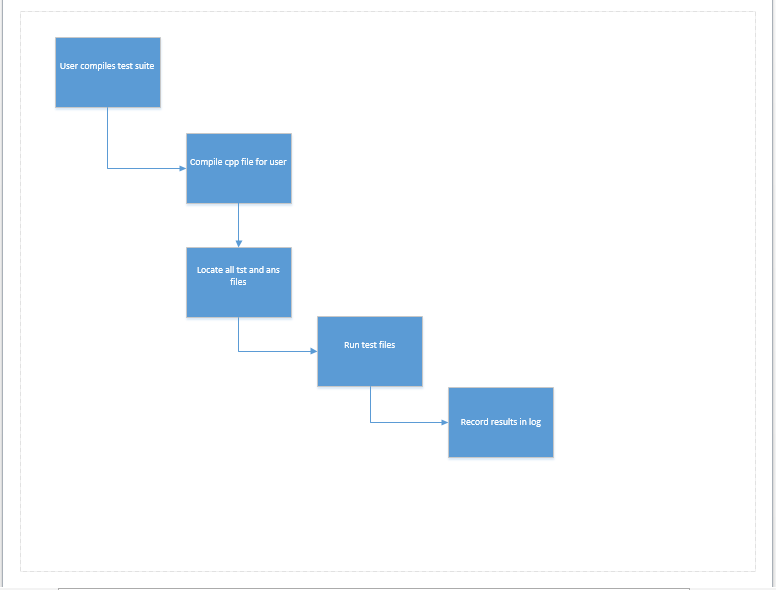
\includegraphics[width=0.75\textwidth]{./Diagran}
\end{center}
\caption{A sample figure .... System Diagram \label{systemdiagram}}
\end{figure}

\section{Technologies Overview}
There was no need for wide range of technologies in this specfic program. However, we have made extensive use of some software to enable us to be productive. Firstly we have used GitHub for version control. We used Trello to keep everybody on track and give an easy place to comunicate job assignments. Finally, but most importantly we used the Linux operating system on the Fujitsu tablets to do all our programing.   
\begin{table}[tbh]
\begin{center}
\begin{tabular}{|r|l|}
  \hline
  7C0 & hexadecimal \\
  3700 & octal \\ \cline{2-2}
  11111000000 & binary \\
  \hline \hline
  1984 & decimal \\
  \hline
\end{tabular}
\caption{A sample Table ... some numbers. \label{somenumbers}}
\end{center}
\end{table}

